%\chapter{Movimientos}
\label{chapter:busqueda}

\subsection{Herramientas software }

Para la programación del robot se necesitaron distintas herramientas de software que permitieron ir desarrollando el comportamiento del robot. A continuación se presenta la descripción de las herramientas utilizadas. 

\begin{itemize}
\item Pypose: Software especializado en el control de los servomotores Dynamixel Ax-12. Una de las más importantes características es que, luego de haber fijado a mano las posiciones de los motores, permite la lectura simultánea de esas posiciones para captar la pose del robot. Con esta herramienta es posible formar una secuencia de poses que generen un movimiento, por ejemplo, caminar. \cite{pypose}

\item ROS: ROS (Robot Operating System) es un framework que proporciona bibliotecas y herramientas para ayudar a los desarrolladores de software a crear aplicaciones robóticas. Proporciona abstracción de hardware,  de dispositivos, bibliotecas, visualizadores, paso de mensajes, gestión de paquetes y más. ROS se encuentra bajo licencia de código abierto, la licencia BSD.

\item OpenCv (Open Source Computer Vision Library): Es una librería de visión de computadoras y aprendizaje de máquinas de código abierto. Ha sido diseñada para acelerar el uso de la percepción de m\'aquinas y para proveer una estructura común en las aplicaciones de visión de computadoras. Registrada bajo la licencia BSD, de código abierto. \cite{opencv}

\item IDE Arduino: Es un entorno de desarrollo para escribir y cargar código en la tarjeta Arduino. Otras tarjetas con microcontroladores AVR también son compatibles, como la ArbotiX. El lenguaje de programación del IDE de Arduino es una implementación de Wiring el cual esta basado en Processing.  \cite{arduino}

\end{itemize}

\section{Busqueda y Pateo}
Como se mencion\'o anteriormente el robot debe buscar y patear una pelota de tamaño de una pelota de tennis y ya se ha descrito las caracter\'isticas f\'isicas y de software que utiliza el robot, esta secci\'n se enfoca en el comportamiento que describe a este robot.
 Para ello primero se especifica la serie de movimientos implementados y el comportamiento que lo representa.

\subsection{Comportamiento}

Debupa es un robot humanoide implemetado de forma autonoma e inteligente que sigue un comportamiento bajo el paradigma h\'ibrido (secci\'on 2 ). El sensor principal (c\'amara ) es el observador del mundo, que posee una serie de movimentos determinados (secci\'on REF) con los cuales escanea el mundo y combinados con la serie de movimiemtos del esqueleto es capaz de encontrar la pelota. Al determinar la posici\'on de la pelota Debupa logr\'o aprender (secci\'on APRENDIZAJE) la mejor acci\'on ha relizar para estar mas cerca de ella y al llegar poder patearla.

Los movimientos tanto de la c\'amara como del esqueleto se explican en las siguientes secciones.  

\subsection{Movimiento del esqueleto}
\label{esqueleto}
El robot debe desplazarse para poder patear la pelota por ello se describen y definen los movimientos del esqueleto que se fueron utilizados.

Con fines explicativos, en este proyecto, la palabra ''pose" se referire a la posición específica de los 16 motores que constituyen el esqueleto del robot. Un conjunto de poses ejecutadas en secuencia se denominará ''acción de movimiento".


Las acciones de movimiento establecidas son:


\begin{itemize}
 \item {Caminar hacia adelante}
 \item {Caminar hacia adelante}
 \item {Caminar hacia adelante}
 \item {Girar a la izquierda}
 \item {Girar a la izquierda} 
 \item {Girar a la derecha}
 \item {Girar a la derecha}	 
 \item {Levantarse cuando ha caído boca abajo}
 \item {Levantarse cuando ha caído boca arriba}
 \item {Patear con la pierna derecha }
 \item {Patear con la pierna izquierda}
 
\end{itemize}

Existen también dos acciones de movimiento que no se encuentran relacionadas con la posición de los motores del esqueleto del robot sino a la posición de los motores que controlan la posición de la cámara. Estas se explicarán en la sección de movimiento de la cámara.

Las poses han sido fijadas a través de la tarjeta controladora Arbotix y el software Pypose. De esta manera se ha fijado y guardado un conjunto de poses para cada acción de movimiento. Estas acciones de movimientos son utilizadas en el programa, en lenguaje Wiring, a ser ejecutado en Arbotix. La programación en Arbotix se ha realizado bajo el ambiente del IDE de Arduino. 


\subsection{Movimiento de la cámara}
La cámara ha sido instalada sobre dos micro servomotores analógicos, otorgándole dos grados de libertad. El servomotor ubicado en la parte inferior se encarga del movimiento horizontal y el superior del movimiento vertical. Las acciones de movimiento relacionadas con el movimiento de la cámara se reduce a 6 posiciones fijas en la figura se puede ver ~\ref{fig:posicionesCam} cuya distribución obedece al objetivo de que la cámara obtenga una amplia visión, sin dejar espacios no visibles. 



\begin{figure}[hbtp]
\label{posicionesCam}
\centering
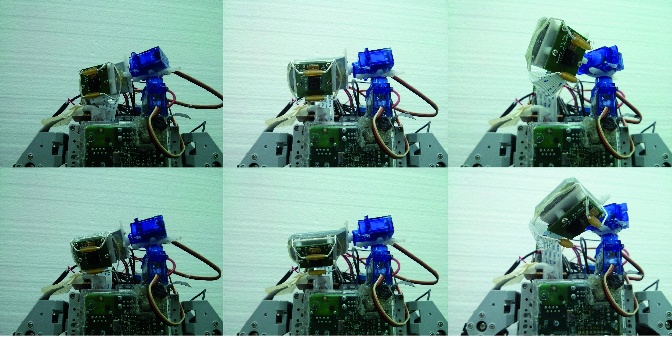
\includegraphics[scale=0.5]{imagenes/Pantallazo.png}
\caption{Posiciones de la cámara }
\end{figure}

Estos motores se controlan desde la Arbotix usando la librería HServo. Esta librería solo puede ser usada para los motores conectados en los puertos Hobby A y B (pines 12 y 13) (ver la figura ~\ref{fig:puertosHobby}). Brinda la ventaja de un control más preciso, evitando que los motores tengan una vibración ya que los pulsos son generados por temporizadores de hardware. 


